\subsection{Descripci\'on del problema}

\noindent
Somos parte del equipo de desarrollo de una web de ventas de pasajes aereos, y queremos ofrecerles a nuestros clientes un servicio que le calcule el itinerario mediante el cual puede llegar de una ciudad, a otra.Se quiere que el itinerario calculado llegue al destino en el menor tiempo posible. Para esto debe evaluar todos los trasbordos necesarios para que el momento de llegada sea minimo. \\
Hay una restriccion que dee cumplirse, en un trasbordo, tiene que haber por lo menos dos horas de diferencia entre la hora de llegada a la ciudad, hasta la salida del proximo vuelo. \\

\subsection{Resoluci\'on}

\noindent
Para resolverlo interpretamos la entrada como un grafo dirigido donde cada ciudad es un vertice, y donde las aristas son los viajes disponibles de una ciudad a otra. \\
Las aristas se definen dinamicamente en el grafo y tienen un costo asociado, correspondiente al costo temporal de viajar de la ciudad $X$ a la ciudad $Y$ m\'as el tiempo de espera desde arrivado a la ciudad $A$.

\noindent
Qu\'e queremos decir con que las aristas se definen dinamicamente?  \\
Empezamos por identificar que el problema es b\'asicamente encontrar un camino m\'inimo entre la ciudad A y B. Pero no podemos simplemente utilizar un algoritmo que resuelva el camino m\'inimo entre esos dos vertices ya que en principio no estamos seguros cuales son las aristas en el grafo. \\

\noindent
Decidimos implementar un Dijkstra modificado que busque el cam\'ino m\'inimo entre dos puntos de un grafo pero tal que vaya completando las aristas entre cada ciertos dos nodos seg\'un los nececite. \\

\noindent
Como resolvemos cuales son las aristas del grafo? \\
Para identificar una arista vamos a tener en cuenta dos cosas: \\
1- Para poder viajar de una ciudad X a una ciudad Y, debe haber una opci\'on de vuelo de X a Y y la hora de arrivo a X debe ser por lo menos 2 horas menor a la hora de salida de la opci\'on de vuelo o X es la ciudad de origen A.\\
2- Si hay m\'as de una opci\'on de vuelo entre una ciudad X y otra ciudad Y, y m\'as de una cumplen el item anterior (1), consideramos tomar como arista la que llegue a Y m\'as temprano. Si llego m\'as temprano a Y tengo igual o m\'as opciones de viaje para el vuelo siguiente. \\

\noindent
Dado un vertice origen, el algoritmo de Dijkstra reutiliza los caminos m\'inimos que ya calcul\'o para calcular contra de vertices no agregados todav\'ia a la solucion. El algoritmo s\'olo se fija aquellas aristas que parten de un vertice del conjunto soluci\'on hacia un vertice que todav\'ia no se encuentre en la soluci\'on. De esta manera podemos adaptar el algoritmo para que incorpore nuevas aristas justo cuando agregue un vertice nuevo a la soluci\'on. Estas aristas por supuesto corresponden a todas las aristas desde el vertice nuevo agregado hacia otros vertices. \\
Para identificar cuales son las aristas nuevas desde el vertice nuevo agregado tenemos en cuenta (1), considerando que la m\'inima hora de arrivo a la ciudad Y es igual al costo del cam\'ino m\'inimo desde X hasta Y, y tenemos en cuenta (2) resultando siempre en definir la arista de menor costo posible.\\

\noindent
La soluci\'on al problema es finalmente el camino m\'inimo entra X e Y calculado por el algoritmo modificado de Dijkstra, que se sigue comportando como Dijkstra, s\'olo que define las aristas del grafo antes de consultar por ellas. \\
\bigskip
\bigskip

\noindent
La resoluci\'on del problema se divide en varias partes:

\begin{itemize}
\item Parsear entrada.
\item Aplicar dijkstraAutofill para busqueda de camino minimo.
\item Obtener solucion del resultado de dijkstra.
\end{itemize}

\noindent
$\proc{Parsear entrada}$ \\

Parseamos la entrada teniendo en cuenta las siguientes estructuras:

\begin{lstlisting}

struct Vuelo{
	Vuelo(int id, int idCiudadOrigen, int idCiudadDestino, Horario inicio, Horario fin);
	int id;
	int idCiudadOrigen, idCiudadDestino;
	Horario inicio, fin;
};

struct Ciudad{
	Ciudad(int id, string nombre);
	int id;
	string nombre;
	list<Vuelo> vuelos;
};

\end{lstlisting}
\bigskip

\noindent
La entrada se parsea un $vector<Ciudad>$, donde el indice es el id de la ciudad. Y el id de la ciudad se define por el orden en que est\'an en la entrada, desde $0$ incrementando en $1$ por cada nueva ciudad.\\
Por cada linea de la entrada se crea una o dos ciudades nuevas, si no existen todavia, y se agregan al vector de ciudades. Despu\'es se agrega el Vuelo que lo describe, a la Ciudad origen.\\
\bigskip

\noindent
pseudoc\'odigo de dijkstraAutofill: \\


\begin{itemize}
\item $\proc{DijkstraAutofill}$
\item V $:=$ $\{0,1,2,...,cantCiudades-1\}$, v $:=$ $0$
\item T $:=$ V - $\{v\}$, $\pi$(v) $:=$ $0$, pred(v) $:=$ $-$1 
\item (*) completar X con las aristas de v
\item $\textbf{para todo}$ u $\in$ V $\textbf{hacer}$
\begin{itemize}
	\item $\textbf{si}$ (v, u) $\in$ X $\textbf{entonces}$
	\begin{itemize}
		\item $\pi$(u) $:=$ costo(v, u), pred(u) $:=$ v
	\end{itemize}
	\item $\textbf{si no}$
	\begin{itemize}
		\item $\pi$(u) $:=$ $\infty$, pred(u) $:=$ $\infty$
	\end{itemize}
\end{itemize}
\item $\textbf{mientras}$ T $\neq$ $\varnothing$ $\textbf{hacer}$
\begin{itemize}
	\item elegir w $\notin$ T tal que $\pi$(w) = $min_{u \in T}$ $\pi$(u)
	\item $\textbf{si}$ no existe tal w 
	\begin{itemize}
		\item $\textbf{END}$
	\end{itemize}
	\item T $:=$ T $-$ w 
	\item (*) completar X con las aristas de w
	\item $\textbf{para todo}$ u $\in$ T y (w, u) $\in$ X $\textbf{hacer}$
	\begin{itemize}
		\item $\textbf{si}$ $\pi$(u) > $\pi$(w) + costo(w, u) $\textbf{entonces}$
		\begin{itemize}
			\item $\pi$(u) $:=$ $\pi$(w) + costo(w, u)
			\item pred(u) $:=$ w
		\end{itemize}
	\end{itemize}
\end{itemize}
\item $\textbf{devuelvo}$ pred
\end{itemize}
\bigskip

\noindent
Codigo de (*) completar X con las aristas de un vertice:

\begin{lstlisting}
void Dijkstra::completarAristas(Vertice v, int horarioLlegada){

  list<Vuelo>::iterator it;
  list<Vuelo>::iterator itIni = (*this->ciudades)[v].vuelos.begin();
  list<Vuelo>::iterator itFin = (*this->ciudades)[v].vuelos.end();
  for (it = itIni; it != itFin; it++){
    
    Vuelo vuelo = *it;
    if (horarioLlegada + 2 <= vuelo.inicio || horarioLlegada == 0){

      G[v][vuelo.idCiudadDestino].completa = true;

      int costo = vuelo.fin - horarioLlegada;
      if (costo < G[v][vuelo.idCiudadDestino].costo){
        G[v][vuelo.idCiudadDestino].id = vuelo.id;
        G[v][vuelo.idCiudadDestino].costo = costo;
      }
    }
  }
}
\end{lstlisting}

\noindent
Tal como explicamos anteriormente completa el grafo incluyendo las aristas de un vertice especifico, iterando sobre los vuelos de la ciudad correspondiente y eligiendo aquellos que representen menor costo y sean posibles de realizar. El horarioLlegada es el costo de llegar al vertice $v$, es decir la hora a la que se arriba a la ciudad que representa el vertice $v$.
\bigskip

\subsection{Complejidad del algoritmo}

Detallamos cada item por separado:

\begin{itemize}
\item Parsear entrada $O(n!)$
\item Aplicar dijkstraAutofill para busqueda de camino minimo $O(n^2)$
\item Obtener soluci\'on del resultado de dijkstra $O(n)$
\end{itemize}


\noindent
$\proc{Parsear entrada}$ \\
La complejidad es 2*O(buscarCiudad) + 2*(O(CrearCiudad)+ O(CrearVuelo)) = O(buscarCiudad) + O(CrearCiudad) + O(CrearVuelo)


\begin{lstlisting}

Vuelo::Vuelo(int id, int idCiudadOrigen, int idCiudadDestino, int inicio, int fin){
	this->id = id;
	this->idCiudadOrigen = idCiudadOrigen;
	this->idCiudadDestino = idCiudadDestino;
	this->inicio = inicio;
	this->fin = fin;
}

Ciudad::Ciudad(int id, string nombre){
	this->id = id;
	this->nombre = nombre;
}

\end{lstlisting}

\noindent
La complejidad de crear un vuelo es O(1) por ser una cantidad finita de operaciones y consultas de int.\\
La complejidad para ver si ya existe una ciudad es O(cantidadCiudades). La cantidadDeCiudades puede ir incrementando como m\'aximo en 2 por cada linea nueva. Y la cantidad de ciudades es como m\'aximo 2n+2.
El resultado es una complejidad de O(2n! + 2) = O(n!). \\
La complejidad de crear una ciudad es O(1+stringCopy), es decir de O(stringCopy). De acuerdo a lo comentado por la catedra rebajamos la complejidad a O(1).\\
La complejidad total luego es la suma de todas las complejidades anteriores = O(1) + O(n!) + O(1) = O(n!)
\bigskip

\noindent
$\proc{DijkstraAutofill}$ \\

\noindent
La Complejidad de dijkstraAutofill es la complejidad del algoritmo defecto de dijkstra m\'as la complejidad de completar las aristas. \\

\noindent
La complejidad de b\'usqueda de cami\'ino m\'inimo de dijkstra es por supuesto O($m^2$) donde m es la cantidad de ciudades. Dado que la cantidad de ciudades est\'a acotada como dijimos anteriormente por 2n+2. La complejidad resulta O($(2n+2)^2$) = O($n^2$) \\

\noindent
La complejidad de completar las aristas es, por cada llamada, recorrer los vuelos del vertice con el que se llama y realizar operaciones O(1) por cada uno. Siempre se llama con un vertice distinto y se hace 1 vez por cada vertice. Entonces la complejidad de esto es O(n).

\noindent
La complejidad total es O($n^2$) +  O($n$) =  O($n^2$)
\bigskip
\bigskip

\noindent
$\proc{Obtener Solucion}$ \\

\noindent
La complejidad es la de recorrer los predecesores de la ciudad destino hasta llegar al origen. C\'omo m\'aximo debe recorrer todas las m ciudades.  \\
Teniendo en cuenta como acotamos m anteriormente, el resultado es una complejidad es O(m) = O(n). 
\bigskip

\noindent
Finalmente la complejidad de todas las partes del algoritmo es O($n^2$). 



\subsection{C\'odigo fuente}

\noindent
C\'odigo de ej1.cpp:

\lstset{language=C++,
                basicstyle=\ttfamily\footnotesize,
                keywordstyle=\color{blue}\ttfamily,
                stringstyle=\color{red}\ttfamily,
                commentstyle=\color{green}\ttfamily,
                morecomment=[l][\color{magenta}]{\#},
                breaklines=true
}
\begin{lstlisting}

#include "ej1.h"

Ej1::Ej1(int idOrigen, unsigned int cantCiudades, vector<Ciudad> &ciudades){

	this->idOrigen = idOrigen;
	this->cantCiudades = cantCiudades;
	this->ciudades = ciudades;
	this->dijkstra = NULL;

}

double Ej1::resolverPlanDeVuelos(int idDestino){
	timespec ts_beg, ts_end;
	clock_gettime(CLOCK_PROCESS_CPUTIME_ID, &ts_beg);


	// BEGIN BIOHAZARD
	if (this->dijkstra == NULL)
		this->dijkstra = new Dijkstra(this->cantCiudades, this->idOrigen, &(this->ciudades));
	this->calcularSolucion(idDestino);
	this->mostrarSolucion();
	// END BIOHAZARD

	cout << "Tiempo de ejecucion: " << endl;
	clock_gettime(CLOCK_PROCESS_CPUTIME_ID, &ts_end);
	double time = (ts_end.tv_sec - ts_beg.tv_sec) + (ts_end.tv_nsec - ts_beg.tv_nsec) / 1e9;
	cout << time << " sec" << endl;
	cout << endl;

	return time;
}

void Ej1::calcularSolucion(int idDestino){

	list<int> vuelosTomados;
	int costoTotal = 0;
	Vertice vertice = idDestino;
	while (dijkstra->damePredecesor(vertice) != -1){
		Vertice predecesor = dijkstra->damePredecesor(vertice);
		vuelosTomados.push_front(this->dijkstra->dameIdArista(predecesor,vertice));
		costoTotal += this->dijkstra->dameCosto(predecesor,vertice);
		vertice = predecesor;
	}

	if (vertice == this->idOrigen){
		this->solucion = std::to_string(costoTotal) + " " + std::to_string(vuelosTomados.size());

		for (list<int>::iterator it = vuelosTomados.begin(); it != vuelosTomados.end(); it++){
			this->solucion += " " + std::to_string(*it);
		}
	}else{
		this->solucion = "no";
	}

}

void Ej1::mostrarSolucion(){
	cout << this->solucion << endl << endl;
};

string Ej1::dameSolucion(){
	return this->solucion;
}

\end{lstlisting}
\bigskip


\noindent
C\'odigo de dijkstraAutofill

\begin{lstlisting}

#include "dijkstra_autofill.h"
#include <cstdlib>
//#include "io.h"


using namespace std;

Dijkstra::Dijkstra(unsigned int cantVertices, Vertice v, vector<Ciudad> *ciudades){
	
	this->ciudades = ciudades;
	this->n = cantVertices;

	generarGrafoSinAristas();

	int *pi = new int[this->G.n];
	this->pre = new Vertice[G.n];
	
	// T : Vertices que no estan en la solucion todavia. a medida que avanza el algoritmo T va decrementando vertices.`
	list<Vertice> T;

	pi[v] = 0;
	
	for (Vertice i=0; i < cantVertices; i++){
		this->pre[i] = -1;
	}

	completarAristas(v, pi[v]);

	for (Vertice u=0; u < G.n; u++){
		if(u==v) continue;
		T.push_back(u);
		if(!G[v][u].completa){
			pi[u] = INF;
		} else {
			pi[u] = G[v][u].costo;
			this->pre[u] = v;
		}
	}
	
	while (!T.empty()){
		Vertice w;
		list<Vertice>::iterator it_w;
		double min = INF;

		for (list<Vertice>::iterator it = T.begin(); it != T.end(); ++it){
			Vertice u = *it;
			if (pi[u] < min){
				w = u;
				it_w = it;
				min = pi[u];
			}
		}

		if (min < INF)
			T.erase(it_w);
		else 
			break; 	
			// El algoritmo termina tambien en caso de que no se encuentren mas nodos que se conecten a los nodos de la solucion.
			// El grafo en este caso no es conexo.

		completarAristas(w, pi[w]);

		for (list<Vertice>::iterator it = T.begin(); it != T.end(); ++it){
			Vertice u = *it;
			if (G[w][u].completa){
				if (pi[u] > pi[w] + G[w][u].costo){
					pi[u] = pi[w] + G[w][u].costo;
					this->pre[u] = w;
				}
			}
		}
	}
}


Dijkstra::~Dijkstra(){
	for (Vertice u=0; u < this->n; u++){
		delete this->pre;
	}
}

void Dijkstra::generarGrafoSinAristas(){

	this->G.n = this->n;
	this->G.ady = new Arista*[this->G.n];

	for (unsigned int i = 0; i < this->G.n; ++i){
		this->G.ady[i] = new Arista[this->G.n];
		for (unsigned int y = 0; y < this->G.n; ++y){
			this->G.ady[i][y].completa = false;
			this->G.ady[i][y].costo = INF;
		}
	}
}


void Dijkstra::completarAristas(Vertice v, Horario horarioLlegada){

	for (list<Vuelo>::iterator it = (*this->ciudades)[v].vuelos.begin(); it != (*this->ciudades)[v].vuelos.end(); it++){
		Vuelo vuelo = *it;
		if (horarioLlegada + 2 <= vuelo.inicio || horarioLlegada == 0){

			G[v][vuelo.idCiudadDestino].completa = true;
			//cout << "G[" << v << "][" << vuelo.idCiudadDestino << "].completa <- true" << endl;


			int costo = vuelo.fin - horarioLlegada;
			if (costo < G[v][vuelo.idCiudadDestino].costo){
				G[v][vuelo.idCiudadDestino].id = vuelo.id;
				G[v][vuelo.idCiudadDestino].costo = costo;
				//cout << "G[" << v << "][" << vuelo.idCiudadDestino << "].id <-" << vuelo.id << endl;
				//cout << "G[" << v << "][" << vuelo.idCiudadDestino << "].costo <-" << costo << endl;
			}
			//cout << endl;
		}

	}
}

int Dijkstra::dameCosto(Vertice v, Vertice u){
	return this->G[v][u].costo;
}

int Dijkstra::dameIdArista(Vertice v, Vertice u){
	return this->G[v][u].id;
}

Vertice Dijkstra::damePredecesor(Vertice v){
	return this->pre[v];
}

\end{lstlisting}
\bigskip


\subsection{Casos de prueba}

\noindent 
Para ejecutar la implementacion del algoritmo con una entrada especifica ejecutamos $ej2/ej2 -p archivoEntrada$

\noindent 
Escogimos particularmente casos de prueba con las siguientes características:

\begin{itemize}

\item Caso sin vuelos hacia la ciudad de destino. En este caso el algoritmo no tiene solucion. ($ej1/recursos/sinVuelosAOrigen1.in$ y $ej1/recursos/sinVuelosAOrigen2.in$)
\item Caso con un vuelo directo de origen a destino. ($ej1/recursos/vueloDirecto1.in$)
\item Caso con un vuelo directo de origen a destino, pero donde la hora de llegada del vuelo directo es mayor a la hora de llegada tomando una via alternativa. ($ej1/recursos/vueloDirecto2.in$)
\item Caso donde hay un vuelo de una ciudad intermedia hasta el destino, pero el vuelo no puede ser alcanzado. ($ej1/recursos/noAlcanzable1.in$ y $ej1/recursos/noAlcanzable2.in$)
\item Caso donde haya 3 o mas vuelos desde una ciudad intermedia al destino y tal que desde el origen pueda volarse a la ciudad intermedia y el primer vuelo no pueda ser alcanzado mientras que el resto si. Debe tomar la mejor opcion de las que queden. ($ej1/recursos/multiplesVuelos.in$)
\item Otros ($ej1/recursos/otro1.in$, $ej1/recursos/otro2.in$ y $ej1/recursos/otro3.in$)

\end{itemize}


\subsection{Performance}

\noindent 
Escribimos un pequenio script llamado graficar.py ($ej1/graficar.py$) cuyo funcionamiento es el de ejecutar tp1ej3 con entradas pseudoaletaorias de $n$ vuelos con $n$ desde 1 hasta 200.000, 300 veces por cada $n$ y con entradas aleatorias por cada repetici\'on. Los parametros de entrada a excepci\'on de $n$ se generan aleatoriamente. Se defini\'o arbitrariamente que las ciudades tienen nombre de numeros y que hay una cantidad de ciudades $m$ igual a un n\'umero aleatorio entre 2 y 2n. Luego las ciudades tienen como nombre 0, 1, 2, 3, ... , $m$. \\
Los horarios de los vuelos se definen tambi\'en de una manera pseudoaleatoria, con horarios de partida directamente proporcional a $n$. \\
(Si para un determinado valor de $n$ las ejecuciones demoran relativamente mucho, el script disminuye las repeticiones para el proximo valor de $n$.) \\

\noindent 
Entendemos que nuestro algoritmo esta acotado por O($n^2$), sin embargo mirando m\'as de cerca la complejidad se parece m\'as a O($m^2+n!$) donde $m$ es la cantidad de ciudades. Tambi\'en a tener en cuenta, que en realidad dijkstra se ejecuta hasta que deje de encontrar vertices conectados al vertice origen. Llamamos M a las ciudades conexas al nodo origen y decimos que entonces la complejidad es todav\'ia m\'as chica a la anteriormente propuesta O($M^2+n!$). \\
Aclaramos esto porque queremos dejar en claro que los tiempos de ejecuci\'on de la implementaci\'on del algoritmo est\'an muy sujetos a parametros de entrada distintos a $n$. Por este motivo existen familias de entradas que pueden mostrar al algoritmo ser parecido a O($n!$), otras a O($n^2$) y otras a complejidades intermedias. \\

\noindent 
Nuestro vamos a corroborar no tanto que el algoritmo propuesto se parezca a O($n^2$) sino que est\'e acotado por esta complejidad. \\

\noindent 
El resultado de los tiempos promedios para cada $n$ se guarda en un archivo llamado resultadosNVariado.dat que contiene por cada l\'inea un valor de $n$ y otro del tiempo promedio que tard\'o en completar la ejecuci\'on de los casos aleatorios para ese n. \\

\noindent 
Usamos estos datos para los gr\'aficos de complejidad pr\'actica contra te\'orica.  \\
El siguiente grafico representa una comparación utilizando escala lineal. \\

\begin{figure}[H]
\begin{center}
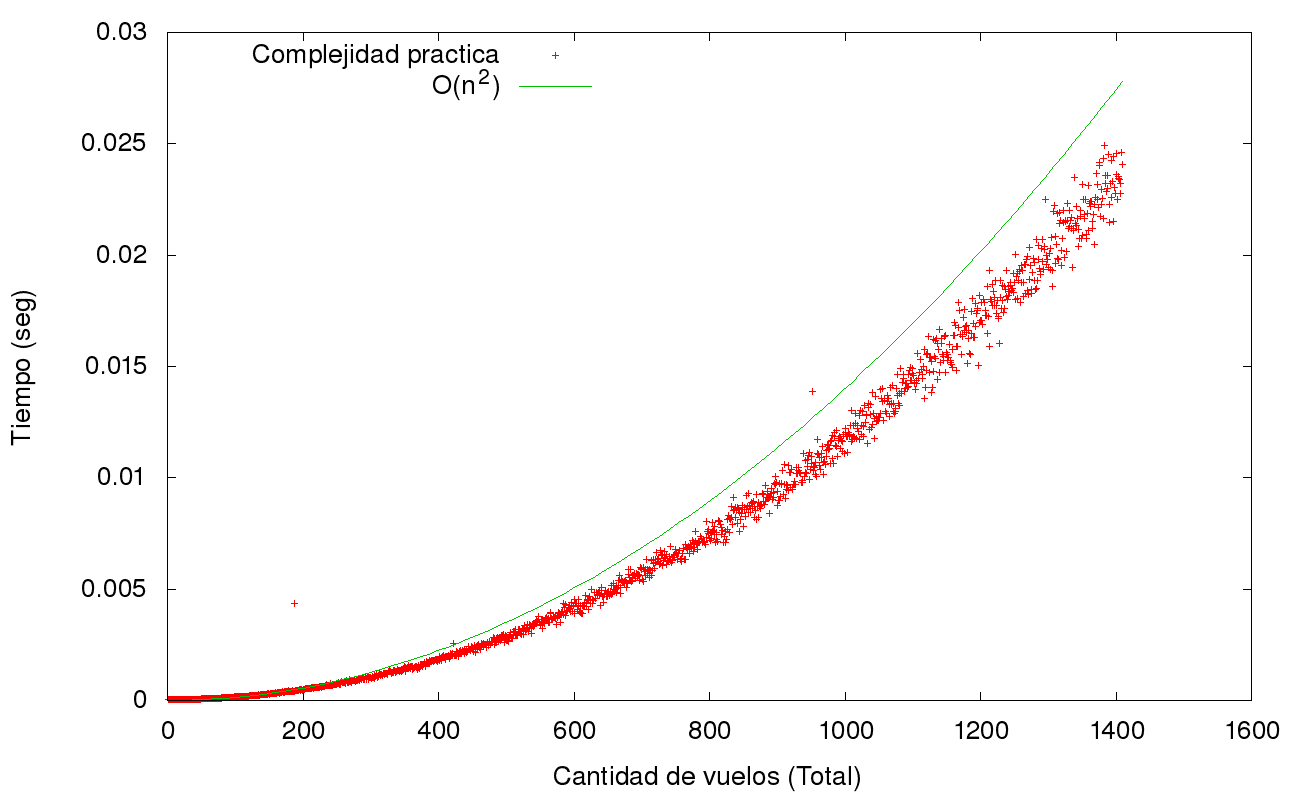
\includegraphics[scale=0.35]{./imagenes/ej1_chartComplejidad.png}
\caption{n variable de 1 a 1400}
\end{center}
\end{figure}

\subsection{Pregunta del RTP 2}

La nueva versi\'on implicar\'ia modificar los parametros de entrada, en cada opcion de vuelo agregar un string que indique la aerolinea del vuelo. Al struct Vuelo entonces le agregariamos por lo tanto el campo string aerolinea que contiene esa informaci\'on. \\
En dijkstraAutofill se debe modificar el c\'odigo de la funci\'on completarAristas. En la misma se debe averiguar cual es el vuelo anteriormente tomado, para esto se chequea el vertice predecesor al recien agregado, y utilizando ambos vertices se averigua el id del vuelo tomado entre ellos. Con el id por supuesto se encuentra la aerolinea utilizada. \\
Luego para cada opci\'on de vuelo desde el vertice recien agregado se chequea la aerolinea utilizada y se realizan los calculos de costo de acuerdo a si coinciden o no. Finalmente que vuelos fueron agregados como aristas depender\'a en parte de las aerolineas a las que pertenece cada vuelo.